%=============================================================================
% Introduction
% Copyright (c) 2018. Lester James V. Miranda
%
% This file is part of thesis-manuscript.
%
% thesis-mansucript is free software: you can redistribute it and/or modify
% it under the terms of the GNU General Public License as published by
% the Free Software Foundation, either version 3 of the License, or
% (at your option) any later version.
%
% thesis-manuscript is distributed in the hope that it will be useful,
% but WITHOUT ANY WARRANTY; without even the implied warranty of
% MERCHANTABILITY or FITNESS FOR A PARTICULAR PURPOSE.  See the
% GNU General Public License for more details.
%
% You should have received a copy of the GNU General Public License
% along with thesis-manuscript.  If not, see <http://www.gnu.org/licenses/>.
%
% Created by: Lester James V. Miranda <ljvmiranda@gmail.com>
%=============================================================================

\chapter{Introduction}
\label{Introduction}

\par In bioinformatics, predicting a protein's function is a fundamental task.
If a protein's functional category is known, then designing drugs or
identifying a disease's molecular mechanism is achievable. However, acquiring
this knowledge is slow and difficult due to the complexity in a protein's
biological information, and the unfamiliarity of life's organization at the
molecular level (\cite{baldi2001bioinformatics}). In addition, more and more
proteins are being characterized by high-throughput sequencing techniques
today, creating vast stores of genomic data available for use
(\cite{gaudet2017gene, cozzetto2017computational}). This widens the gap between
annotated and unannotated proteins, urging the need for a more efficient,
accurate, and fast set of prediction techniques in the presence of
``genomic big data.''

\par Machine learning techniques have been observed to perform well in complex
tasks involving large amounts of data (\cite{chen2014data}). They have been
exceptional in recognizing patterns and learning from a vast number of examples 
(\cite{lecun2015deep}). Before prediction, a machine learning model must first
discern a pattern from a set of data, and use that to infer the category, or 
\textit{class}, a new sample belongs to. Because most proteins can perform
multiple functions at once, \textit{multi-label classification}\textemdash
a subset of machine learning\textemdash is used. However, the effectiveness of
a multi-label classification model still depends on the pattern it learns, and
how well it represents the input data provided.

\par Learning to understand data and representing it in a form beneficial for a
machine learning model is known as \textit{representation learning}. Although
it is entirely possible to manually engineer characteristics, or \textit{features}
, of a dataset, it is labor-intensive and requires thorough domain-expertise 
(\cite{bengio2013representation}).  Instead, it is preferable to automatically
extract useful information from data using a \textit{feature extractor}, and
ensure that the new features are relevant. Selecting more relevant features is
apt for protein datasets because it is noisy, i.e., both relevant and irrelevant
data are present. Properly discerning which characteristics are important and 
transforming them into features useful to a predictor is essential in
identifying protein functions.

\par This research presents a novel architecture based on the autoencoder neural
network. The proposed network motivates selective behavior in order to produce
relevant features. This is done through mutual competition: adjusting the
backpropagation path to keep a select number of neurons active while ensuring
meaningful representations. It is expected that this method will be able to
predict protein functions well, as compared to using raw data directly or to
other techniques in literature. 

\newpage

\par \noindent The rest of the document is organized as follows:

\begin{itemize} 
    \item The remaining sections of Chapter \ref{Introduction}
        discuss the context behind this work (Sec. \ref{Background}), the
        research motivation (Sec. \ref{Motivation}), and the formulation of the
        research problem (Sec. \ref{Problem}).  
    \item Chapter \ref{LiteratureReview} comments on the related literature
        that also tackles the problem of protein function prediction. 
    \item Chapter \ref{Methodology} outlines the proposed method
        and gives an overview of its training and testing schemes (Sec. 
        \ref{Overview}). In addition, an explanation of the datasets used (Sec.
        \ref{Datasets}) and a description of the experimental environment
        (Sec. \ref{ExperimentalEnvironment}) will be done. 
    \item Chapter \ref{Results} discusses the experiments conducted to evaluate the 
        proposed method: benchmarking performance with other techniques 
        (Sec. \ref{Benchmarking}), measuring model quality (Sec.\ref{ModelQuality}),
        and estimating feature relevance (Sec.\ref{FeatureRelevance}).
    \item Lastly, Chapter \ref{Conclusion} concludes the work. Potential avenues for 
        future research (Sec. \ref{FutureWork}) will be discussed.
\end{itemize}


\section{Background of the Study}
\label{Background}

Approaching the problem of protein function prediction requires the
understanding of how protein data is represented. Proteins are always
described into two: first by their (1) \textbf{features} or characteristics,
and second by their (2) \textbf{labels} or set of functions it performs. This
section will discuss these types of data, and give a brief background on two
related topics: \textbf{multi-label classification}, a set of machine learning
methods for predicting multiple associations in a sample, and \textbf{feature 
extraction}, a technique for finding new representations from raw data.

\subsection{Protein features}

\par Proteins can be described into either sequences or expressions 
(\cite{xiong2006essential}). Sequences describe the protein as a chain
of amino acids, the building blocks of protein, represented by a single letter.
When arranged into a sequence, the order of appearance becomes important.
On the other hand, expressions describe the protein as combinations of various
techniques such as micro-array expression data, phylogenetic profiles and DNA
chips. It represents proteins as a vector of numerical values containing the
output of the micro-array process.

\par Although prediction is possible using protein sequences
(\cite{whisstock2003prediction, devos2000practical}), expressions have
been observed to be effective in predicting protein functions
(\cite{eisenberg2000protein, marcotte1999combined}). Thus, this
research will focus on the latter as descriptors for protein data. In
particular, micro-array expression data and phylogenetic profiles will
be used (See Sec. \ref{Datasets})

\subsection{Protein functions}

\par Proteins can belong to one or more functional categories. They
refer to various life processes such as metabolism, cell
reproduction, synthesis that arranged in an ontology. This
organization enables researchers to observe the relationships and 
properties of protein functions, and is one of the standard tools
in bioinformatics today.

\par Various ontologies describe a protein's functional category,
and two of the most common are the Gene Ontology (GO) and the Munich
Information Center for Protein Sequences (MIPS) annotations
(\cite{gaudet2017gene, mewes2006mips}). Although each differ on their
experimental methods, they remain similar by representing
protein functions as a direct acyclic graph (DAG) to express the relationship
between its members (e.g., ``is-a'', ``part-of'', etc.). To illustrate,
Figure \ref{demo:yeast_go} shows the gene ontology of the  function ``cellular
bud site selection'' performed by YAL041W, a protein found in
\textit{S. cerevisiae} or baker's yeast.

\begin{figure}[!t]
  \centering
  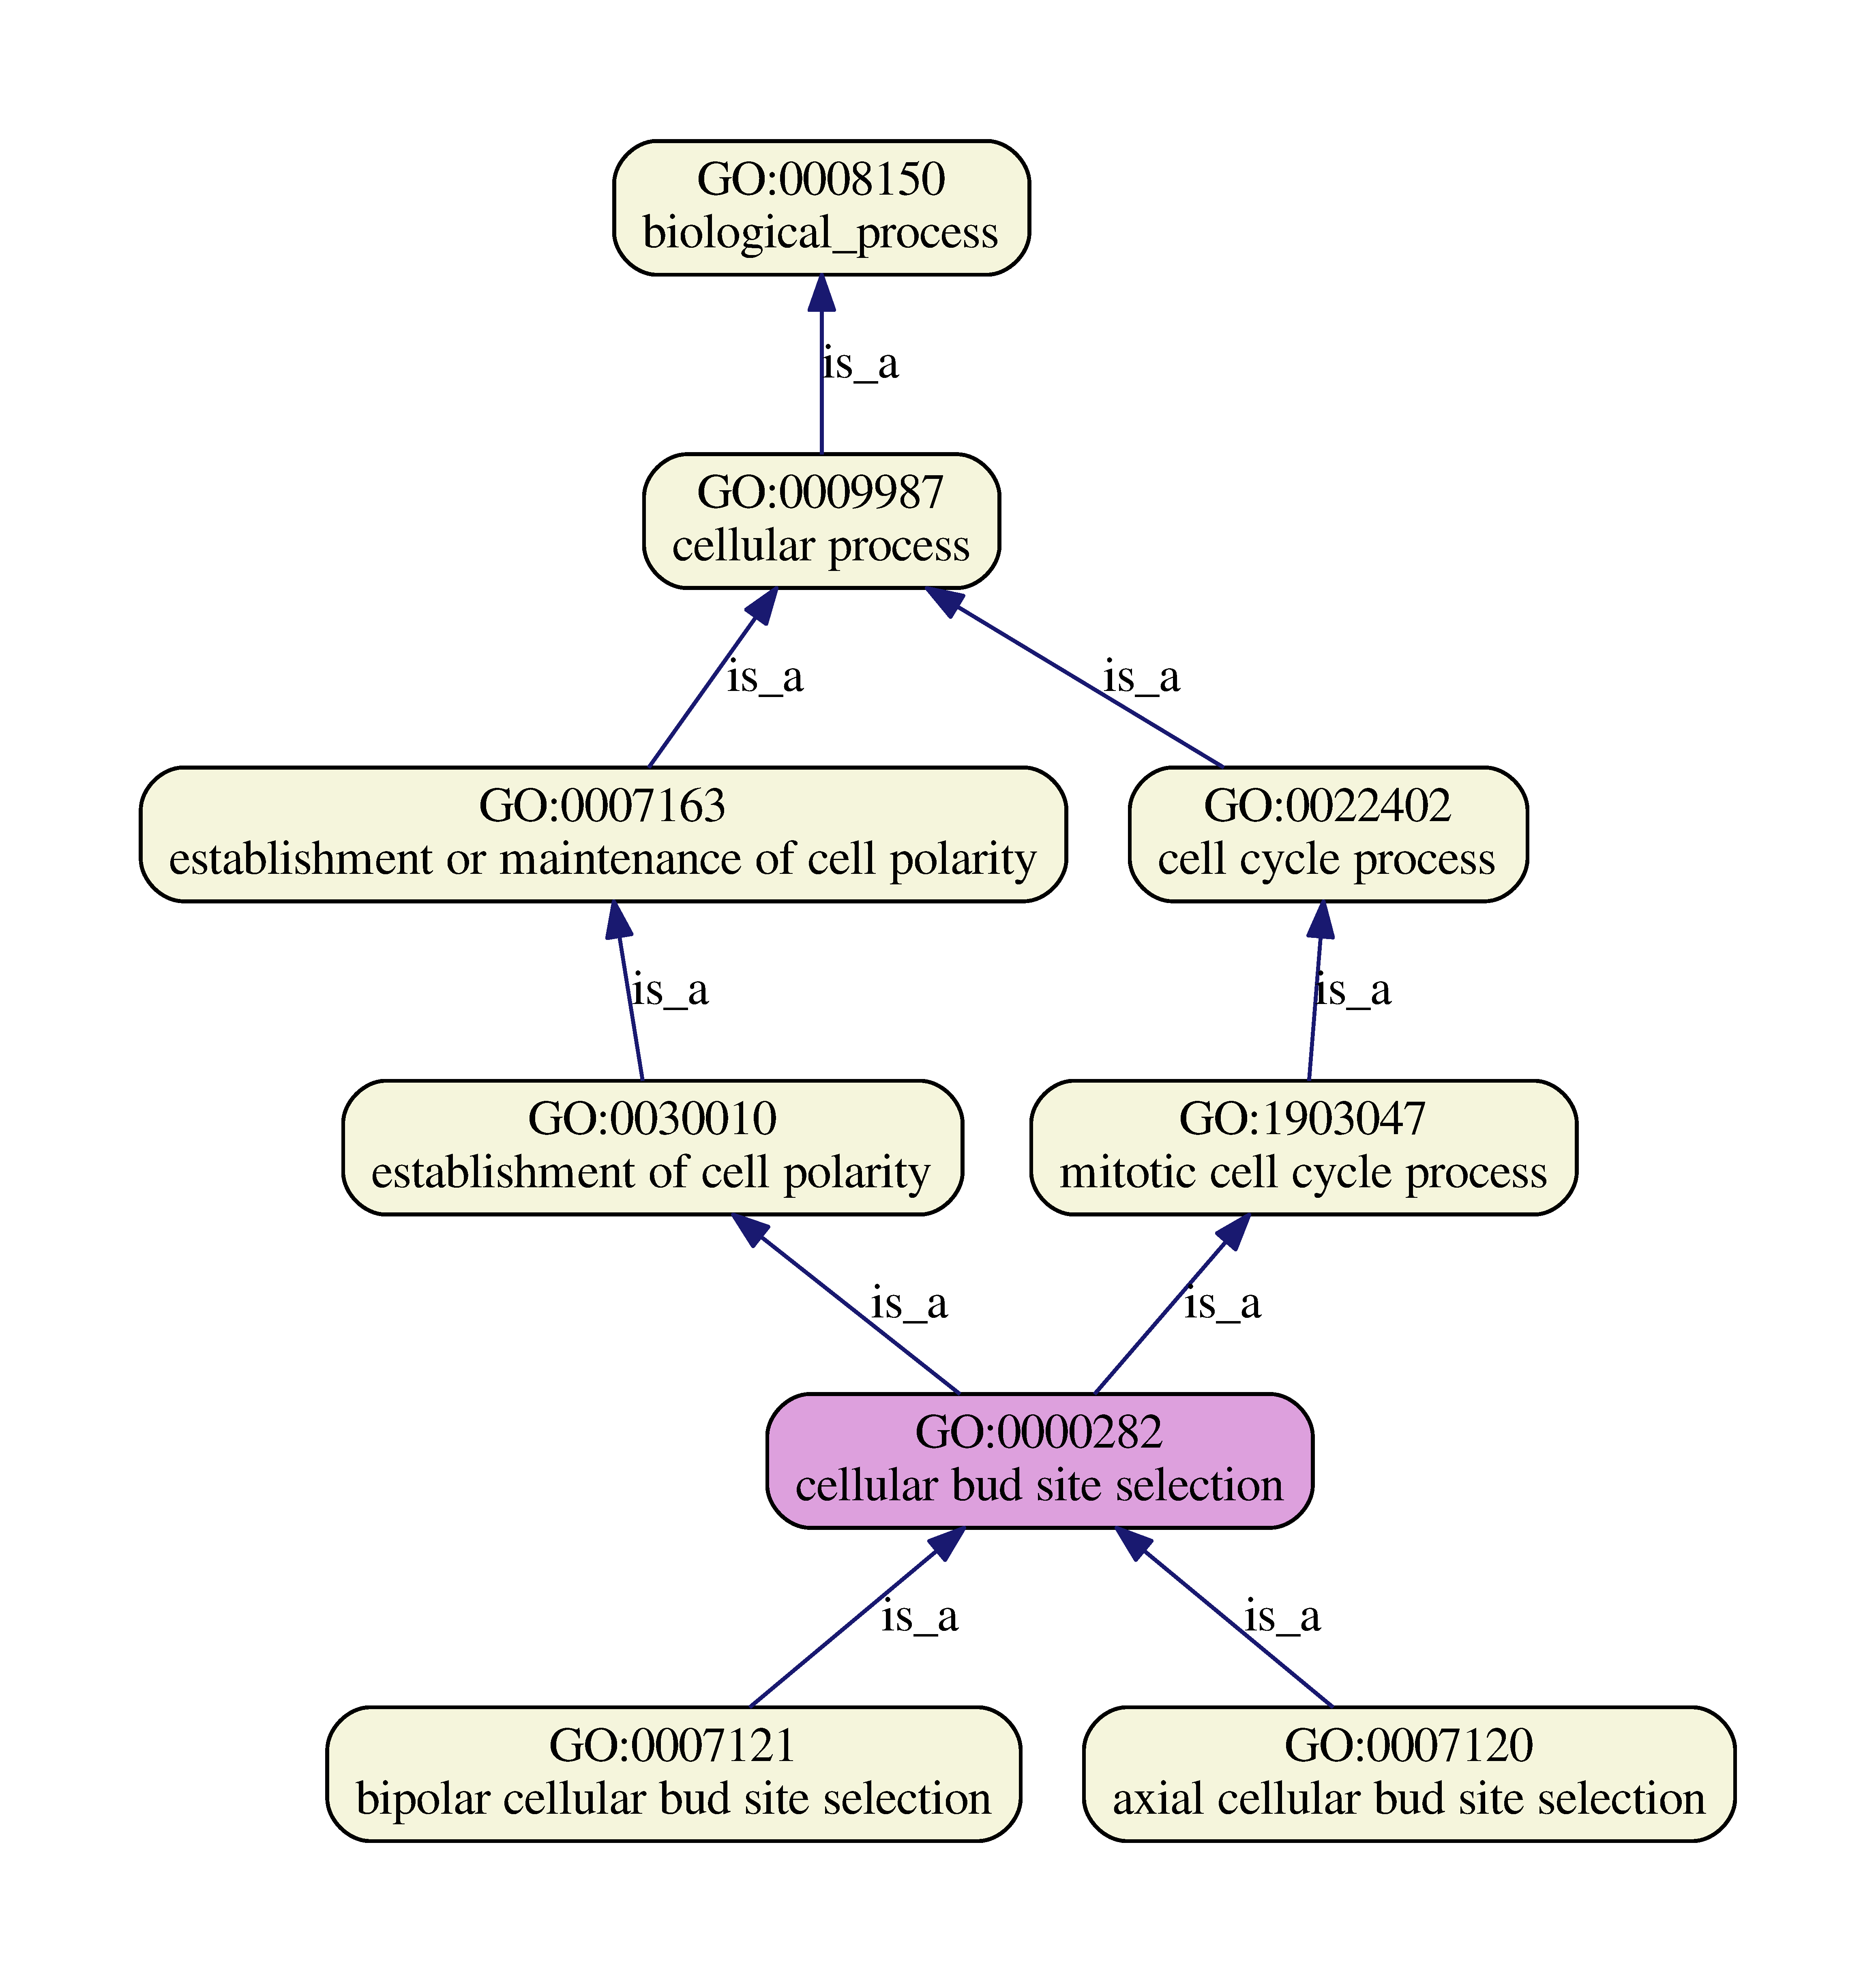
\includegraphics[width=0.49\textwidth]{ch01/demo_lineage}
  \caption[Gene ontology for \texttt{GO:0000282} or "cellular bud site selection"]{
      Gene ontology for cellular bud site selection (\texttt{GO:0000282})
      showing its relationship with respect to the parent and child classes.
  }
  \label{demo:yeast_go}
\end{figure}

\par It is evident from \texttt{GO:0000282}'s ontology that hierarchical
relationships exist between protein functions. This research strictly
focuses on multi-label classification without accounting for label
hierarchy. The benchmark datasets employed in this work and in existing literature
have independent, multiple labels. Still, classification in the presence
of multiple labels is no trivial task, and it is important to understand common 
techniques for overcoming this problem.

\subsection{Multi-label classification}

\par In typical classification tasks, two kinds of data are presented:
the \textit{features}, denoted by the matrix $\mathbf{X} =
(\mathbf{x}_{1}, \mathbf{x}_{2}, \dots, \mathbf{x}_{N})$, describing
a measurable characteristic from the system being observed, and the
\textit{labels}, denoted by the matrix $\mathbf{y} = (y_{1}, y_{2}, \dots
y_{N})$, categorizing the features into classes. A sample $i$
can be defined as a joint feature-label pair $(\mathbf{x}_{i}, y_{i})$ and a
dataset $D$ with $N$ samples can then be described as $N$ pairs of feature
and label vectors  $\{(\mathbf{x}_{i}, y_{i})\}_{i=1}^{N}$.

\par Labels are scalar values $y_{i} \in \{0, 1, 2, \dots C\}$ where each digit 
corresponds to a particular class (e.g. for image classification, $0$ is
``person'', $1$ is ``sea'', $2$ is ``boat'' and so on). The goal of
classification is to learn a hypothesis function $h$ such that it minimizes a
cost function $J$. Recall that in this task, only a single class is associated
to a particular sample. Clearly, this does not represent the case of proteins,
given that multiple classes are associated to it. Imagine a picture of a beach:
one can observe not only the ``sea'' nor the ``person,'' but both of them
existing in the same image as shown in Figure \ref{demo:multilabel}.

\begin{figure}[!t]
  \centering
  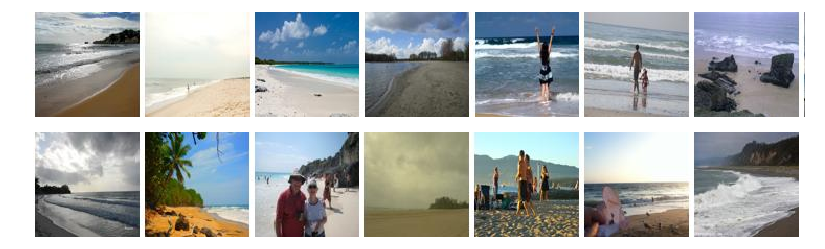
\includegraphics[width=0.70\textwidth]{ch01/demo_multilabel}
  \caption[Example of multi-label data in image scenes from MIT
  Places dataset]{
      Example of multi-label data in image scenes from the MIT
      Places dataset (\cite{zhou2014learning})}
  \label{demo:multilabel}
\end{figure}

\par For multi-label datasets, labels are often defined by vectors instead of
scalars. Here, the notation $\mathbf{Y}$ denotes the whole label matrix
containing $\mathbf{Y} = (\mathbf{y}_{1},\mathbf{y}_{2}, \dots,
\mathbf{y}_{N})$ labelsets for all samples $N$. Each sample $i$ is now defined
by a joint pair of vectors $(\mathbf{x}_{i}, \mathbf{y}_{i})$ rather than a
vector-scalar as seen in a single-label classification task. Thus for each
labelset $\mathbf{y}_{i}$ of size $L$, there exists $\mathbf{y}_{i} =
(\lambda_{1}, \lambda_{2}, \dots, \lambda_{L})_{i}$ where $\lambda_{l} \in \{0,
1\}$. The value $L$ corresponds to the number of possible labels $\lambda_{l}$
in the whole dataset. For a given protein sample, a value of $\lambda_{l}=1$
means that it performs the function $l$, whereas $\lambda_{l}=0$ means
otherwise.

\par There are two main approaches in classifying multi-label data: first by
\textit{problem transformation}, where a multi-label problem is transformed
into separate single-label classification tasks, and the second is
\textit{algorithm adaptation}, where a classifier is designed to 
directly handle multi-label data (\cite{tsoumakas2007multilabel}). This
research will focus on problem transformation, primarily because it is easier
to treat the classifier and the feature extractor as separate modules: the
classifier can be de-coupled from the feature extractor, enabling the former
to be tested on different variants of the latter.  Another reason is that the
literature on problem transformation techniques is extensive enough to
enable benchmark comparisons with different multi-label classifiers in the
future (\cite{zhang2014review, madjarov2012extensive}). The extent
of this work focuses on a specific technique called \textbf{binary relevance},
and will be treated as the baseline during the experiments.

\par Binary relevance (BR) is a problem transformation technique that
decomposes a multi-label problem into a series of single-label classification
tasks (\cite{boutell2004learning, tsoumakas2007multilabel}). This means that a
classifier $h$ is trained on each label $\lambda_l$ of $\mathbf{Y}$, training
a total of $L$ classifiers. Further modifications can be done to binary
relevance such as training a combination of labels, or building chains of
classifiers (\cite{read2009classifier}). However, due to BR's conceptual
simplicity and time-complexity\footnote[2]{
    Most problem-transformation techniques have an overhead time-complexity
    depending on the classifier $h$. For Binary relevance, we have $\bigO(L
    \cdot h(N, M))$. At inference, the complexity is $\bigO(L
    \cdot h'(M))$. This is relatively faster compared to Classifier Chains
    $\bigO(L \cdot h(N, M + L))$ or Label Ranking $\bigO(L^{2} \cdot h(N, M))$
    (\cite{zhang2014review}).
}, it has been widely used
in most literature (\cite{zhang2017binary}).

\par This research will concentrate on finding good representations for the
binary relevance classifier to solve the problem of protein function
prediction. Specifically, a binary relevance Support-Vector Machine (SVM) will
be utilized. This process of obtaining new features from raw data is called 
\textit{feature extraction} and will be one of the core ideas in this work. Even
if a BR classifier can stand on its own, it is hypothesized that higher
performance is achievable when using the extracted features as compared to the
raw data itself.

\subsection{Feature Extraction}

\par Feature extraction can be best illustrated with the \texttt{XOR} gate.
Here, we take its two inputs $\mathbf{x}_{i} = (x_{1}$, $x_{2})_{i}$ as features
and its output $y_{i} \in \{0,1\}$ as the label. With $N=4$ samples
representing all possible bit-combinations, a ``dataset''
$D=\{(\mathbf{x}_{i}, y_{i})\}_{i=1}^{4}$ can be constructed as:

\[
    D = \{(0,0,0), (0,1,1), (1,0,1), (1,1,0)\}
\]

Assuming we only have access to a linear classifier, the feature-space shown
in Figure  \ref{demo:xor} (\textit{left}) proves that classifying the samples is
difficult due to its linear inseparability\textemdash that is, drawing a single
line to perfectly separate the \texttt{X}'s and \texttt{O}'s is impossible.
However, if a new feature-space $\mathbf{\widehat{x}}$ is engineered in such a
way that $\mathbf{\widehat{x}} = (\widehat{x}_{1}, \widehat{x}_2)$ where 
$\widehat{x}_{1} = \text{\texttt{AND}}(\bar{x}_{1}, x_{2})$ and $\widehat{x}_{2}
= \text{\texttt{AND}}(x_{1}, \bar{x}_{2})$, then it is possible to transform $D$
into dataset $\widehat{D}=\{(\mathbf{\widehat{x}}_{i}, y_{i})\}_{i=1}^{4}$
where:

\[
    \widehat{D} = \{(0,0,0), (1,0,1), (0,1,1), (0,0,0)\}
\]

\noindent it can be seen from Figure \ref{demo:xor} (\textit{right}) that 
$\widehat{D}$ is a linearly separable problem solvable by any simple classifier.
In this demonstration, it is evident that hand-engineering features, or
\textit{extracting new features} has been helpful. However, with large
datasets, it will be tedious to manually find useful representations from data.
It is much preferred to automate the whole process. Note that  using this
technique is similar to finding a direct encoding from raw inputs to their 
representation. If there is no context of $\mathbf{\widehat{x}}$'s form, then
there's a need to learn a function $f$ such that $f: \mathbf{x} \rightarrow 
\mathbf{\widehat{x}}$.

\begin{figure}[!b]
  \centering
  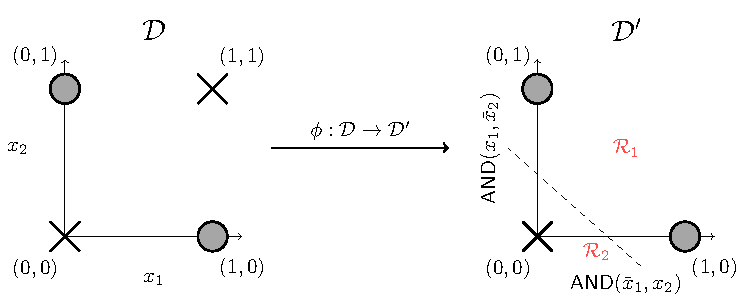
\includegraphics[width=0.70\textwidth]{ch01/demo_xor}
  \caption[Illustration of feature extraction using the \texttt{XOR} gate]{
      Illustration of feature extraction using the \texttt{XOR} gate. Using the
      raw data gives us a linearly inseparable problem \textit{(left)}.
      Constructing new features from raw data transforms the problem into a
      linearly separable one \textit{(right)}
  }
  \label{demo:xor}
\end{figure}

\subsubsection{The basic autoencoder}


\par This research proposes a feature extraction technique based on the
autoencoder neural network. As a prerequisite, it is necessary to understand
how a basic autoencoder shown in Figure \ref{schema:autoencoder} works.
Here, the function $f$ is obtained by learning a parametric map that directly
encodes the inputs to their representation (\cite{hinton1994autoencoders}).
This method relies on the features $\mathbf{X}$, unlocking correlations and 
relationships that may not be easy to find manually. The literature considers
this kind of technique as \textit{unsupervised learning} 
(\cite{bengio2013representation}).

\par Given a feature set $\mathbf{X}$, the aim is to find a set of parameters
$\theta$ such that the composite function $(g_{\theta'} \circ f_{\theta})
(\mathbf{X})$ minimizes the reconstruction error:

\[
    J(\theta) = L(\mathbf{X}, g_{\theta'}(f_{\theta}(\mathbf{X})))
\]

\noindent Here, the functions $f$ and $g$ are known as the encoder and decoder.
The former encodes the data into a representation $\mathbf{h} = f_{\theta}
(\mathbf{X})$ while the latter attempts to reconstruct $\mathbf{h}$ back into 
$\mathbf{X}$ via $\mathbf{\widetilde{X}} = \mathbf{X} \approx g_{\theta'}
(\mathbf{h})$. Most works implement a tied-weighing scheme (i.e,
$\theta=\theta^{T}$ between the encoder and decoder weights
(\cite{bengio2013representation}). Take note that the
size of $\mathbf{h}$ may not necessarily be the same as $\mathbf{X}$. In sum,
the autoencoder takes an input matrix and faithfully reconstructs it given a
bottleneck (the size of $\mathbf{h}$). This may sound trivial, but due to the
\textit{encoding layer}  $\mathbf{h}$, interesting structure is learned from
the data. The learned representations $\mathbf{h}$ are treated as the new
input $\mathbf{\widehat{X}}$  (similar to the \texttt{XOR} problem) for a
classifier. With a good set-up and optimization scheme, it is even possible to
compress data using this technique (\cite{theis2017lossy}).

\begin{figure}[!t]
  \centering
  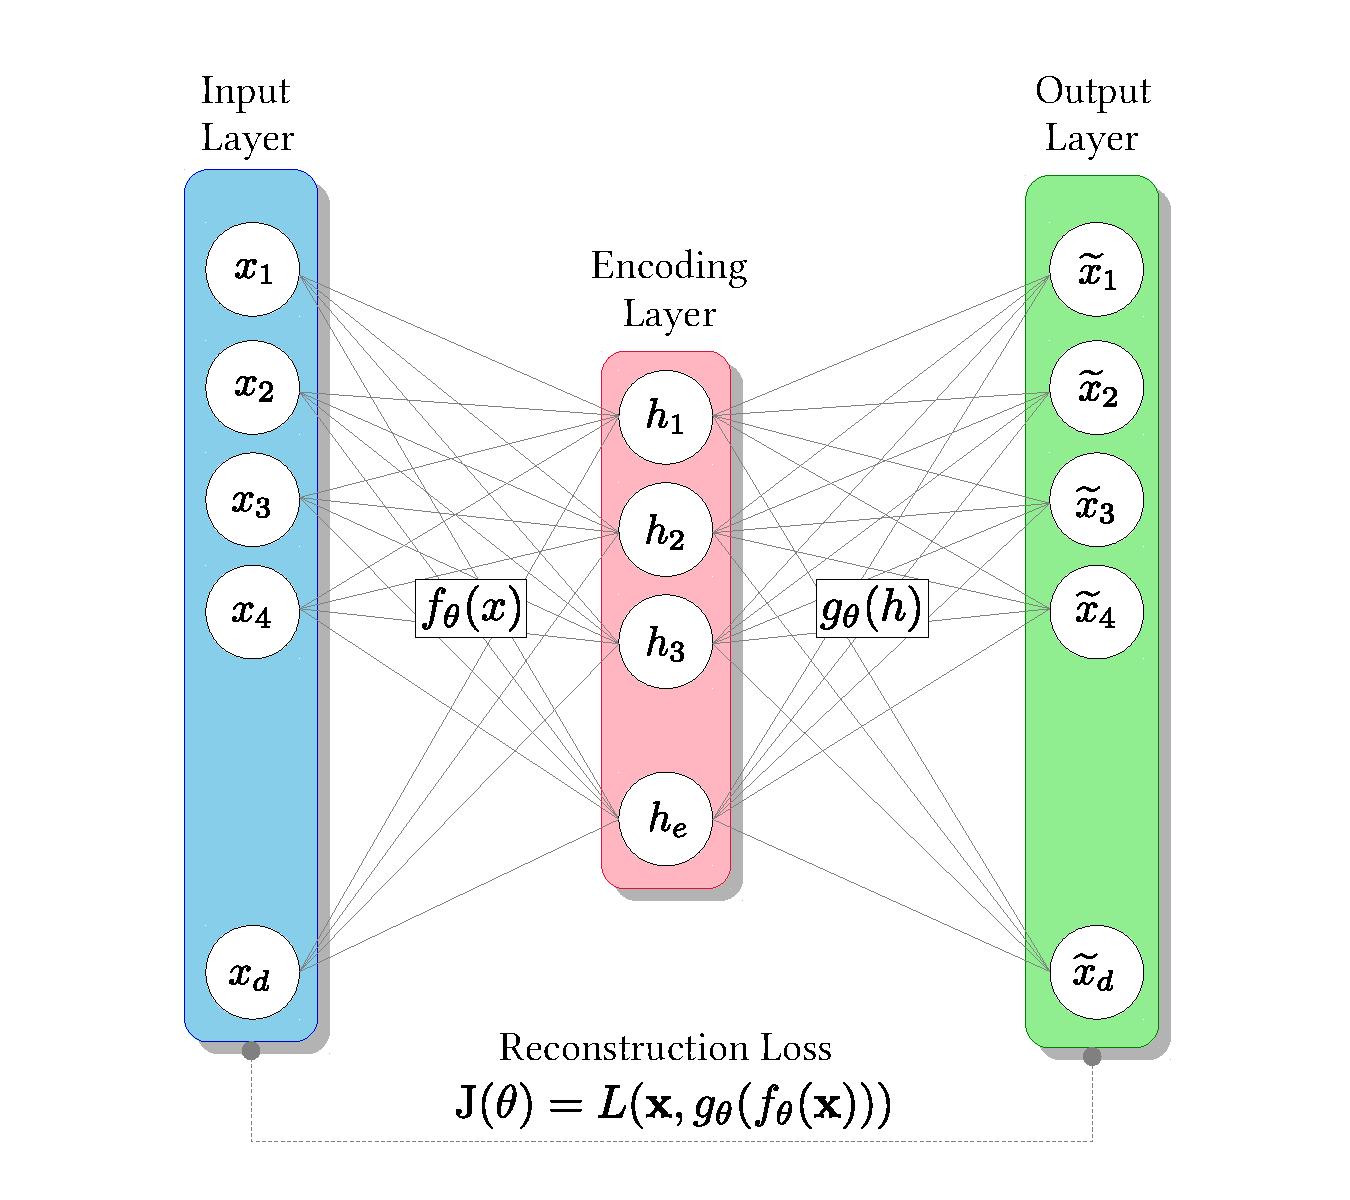
\includegraphics[width=0.60\textwidth]{ch01/schema_autoencoder}
  \caption[Diagram of the basic autoencoder]{
      Diagram of the basic autoencoder
  }
  \label{schema:autoencoder}
\end{figure}

\section{Motivation}
\label{Motivation}

\par Although extracting features using an autoencoder has been helpful for
classification, one shortcoming of this technique is its tendency to learn
trivial representations from sparse and high-dimensional data
(\cite{wang2017feature, chen2017kate})\textemdash types of data characteristic
of proteins. This is usually the case when the optimization task is to learn
an approximation to the identity $\mathbf{X} \approx \mathbf{\widehat{X}}$,
favoring irrelevant features by overfitting instead of learning a generalized
pattern or representation. Motivating the autoencoder to create relevant features
for the classification task is then important.

\par To address this issue, this work proposes an autoencoder architecture that
extracts a set of sparse yet relevant features. This is done through mutual
competition: the neurons on the network compete based on their activation, and
the ``winners'' absorb the ``losers,'' boosting their importance in the network.
Competition adjusts the backpropagation path, favoring the winners to represent
the input data. This method is task-specific for protein data because only a subset
of its features is considered useful (\cite{iqbal2014efficient, gaudet2017gene}).
The proposed method will be trained on two protein benchmark datasets, and the
extracted features will be used as input to a binary relevance classifier. It will
be compared against a baseline method without feature extraction, and opposed to
existing techniques in literature.

\section{Problem Formulation}
\label{Problem}

\par This research proposes a technique for extracting relevant features from
protein data. It also investigates the effect of feature-relevance to the
performance of a multi-label classifier. Selective feature extraction is
accomplished by encouraging competition between the neurons of an
autoencoder network. In line with this, the following questions will be
answered throughout this work:

\begin{itemize}
    \item How relevant are the learned representations from the proposed method
        as compared to the raw features? (Sec. \ref{FeatureRelevance})
    \item How well does a multi-label classifier perform when using the
        features extracted by the proposed method? (Sec. \ref{ModelQuality})
    \item How well do the hyperparameters improve the basic autoencoder and
        affect model performance? (Sec. \ref{AblationTest})
    \item How well does the proposed method compare with other techniques in
        literature? (Sec. \ref{Benchmarking})
\end{itemize}


